\documentclass{article}

%\usepackage{mathtools}
\usepackage{amsfonts}
\usepackage[spanish,mexico]{babel}
\usepackage[utf8]{inputenc}
\usepackage{graphicx}
\usepackage{booktabs}
\usepackage{url}
\usepackage{listings}%http://www.tex.ac.uk/FAQ-codelist.html
\usepackage{color}

\definecolor{codegreen}{rgb}{0,0.6,0}
\definecolor{codegray}{rgb}{0.5,0.5,0.5}
\definecolor{codepurple}{rgb}{0.58,0,0.82}
\definecolor{backcolour}{rgb}{0.95,0.95,0.92}

\lstdefinestyle{mystyle}{
  backgroundcolor=\color{backcolour},
  commentstyle=\color{codegreen},
  keywordstyle=\color{magenta},
  numberstyle=\tiny\color{codegray},
  stringstyle=\color{codepurple},
  basicstyle=\footnotesize,
  breakatwhitespace=false,
  breaklines=true,
  captionpos=b,
  keepspaces=true,
  numbers=left,
  numbersep=5pt,
  showspaces=false,
  showstringspaces=false,
  showtabs=false,
  tabsize=2
}

\lstset{style=mystyle}
\graphicspath{ {img/} }
%\usepackage{enumitem}
%\usepackage{tikz}

\title{Densidades y distancias promedio de grafos ciclos a completos}
\author{José Alberto Benavides Vázquez}
\date{\today}

\begin{document}

  \maketitle

  Esta práctica se realizó a partir de un programa en desarrollo para flujo en redes alojado en \url{https://github.com/jbenavidesv87/FlujoRedes}. El código de esta práctica puede consultarse en \url{https://github.com/jbenavidesv87/FlujoRedes/tree/master/ejemplos/07Densidad} \cite{Grafos}.

  \section{Introducción}

  Un \textbf{grafo ciclo} es un grafo en el que sus $n$ nodos están conectados uno tras otro, sin repeticiones, salvo por el úlitmo nodo que se conecta al primero para formar una figura que se asemeja a un polígono de $n$ lados. Por su parte, un \textbf{grafo completo} es un grafo ciclo en el que sus $n$ nodos están conectados con los restantes $n - 1$ nodos. En cuanto a las aristas, los grafos ciclo tienen la mínima cantidad de aristas necesarias para cumplir su definición y formar un ciclo, esto es $a = n$ aristas; mientras que los grafos completos poseen todas las aristas posibles que pueden establecerse sin repetir pares de nodos entre sí, a saber $a = n \cdot (n-1)/2$ aristas. A partir de estas descripciones, se puede definir un valor $k$ que especifique la cantidad de nodos vecinos con los que se conectará cada nodo de este tipo de grafos por cada uno de sus costado. Este valor $k$ puede tomar valores enteros del intervalo $[1, \lfloor n / 2 \rfloor]$. Por ejemplo, un grafo con seis nodos podría tener $k = \{ 1, 2, 3 \}$ que corresponden a $\{ 6, 12, 15 \}$ aristas en un polígono de 6 lados, como se puede constatar en la figura \ref{grafoEjemplo6} (p.\pageref{grafoEjemplo6}).

  \begin{figure}[h]
    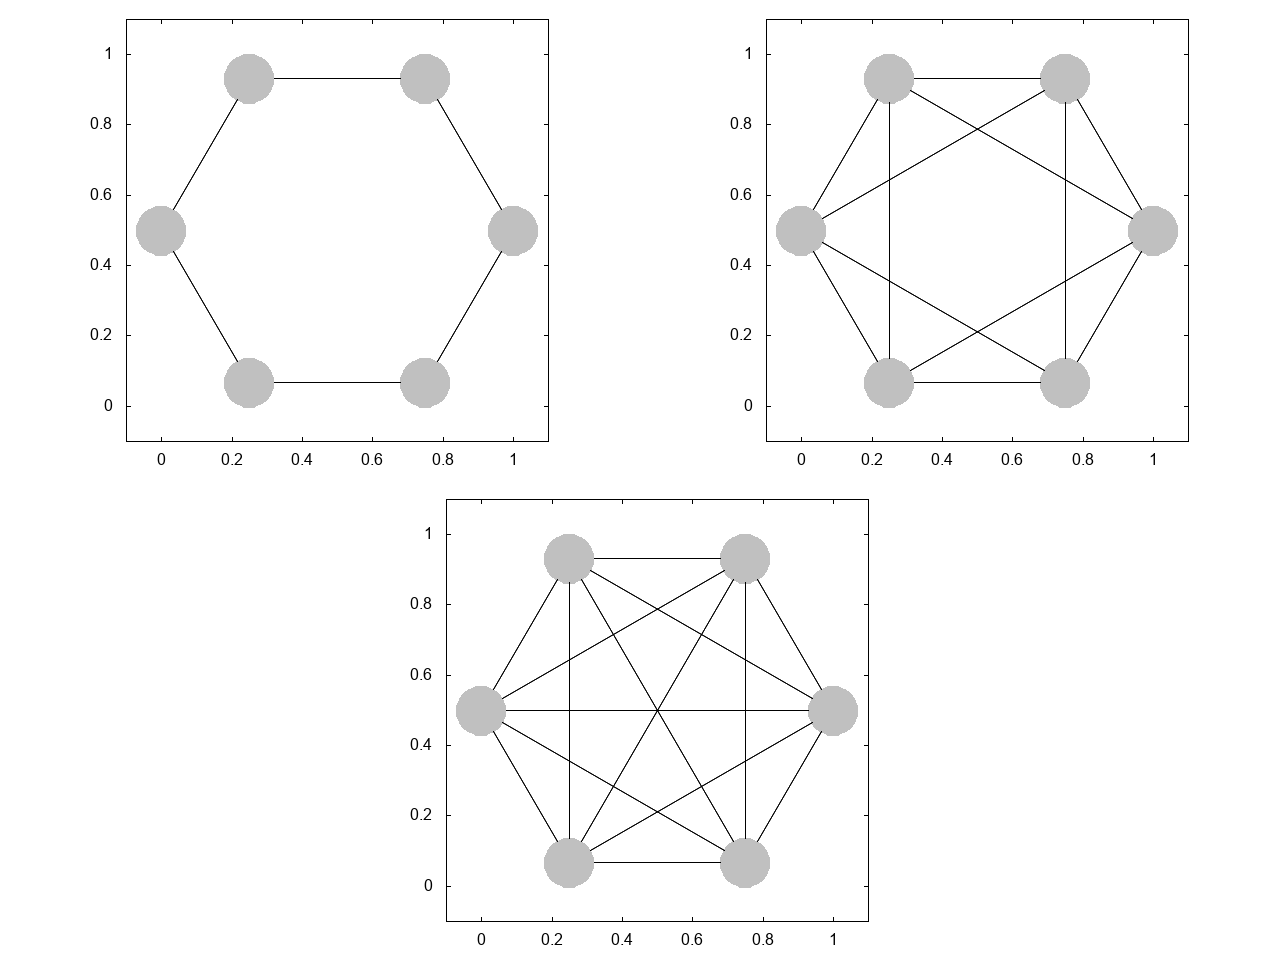
\includegraphics[width=1\textwidth]{grafoEjemplo6}
    \centering
    \caption{En orden izquierda, derecha y abajo, grafos de seis nodos con $k = \{ 1, 2, 3 \}$ y $\{ 6, 12, 15 \}$ aristas.}
    \label{grafoEjemplo6}
  \end{figure}

  Para esta práctica se ha desarrollado un programa que genera grafos de este tipo a partir de la definición de la cantidad de nodos y del valor $k$. A manera de ejemplo, se creó una animación de un grafo de cuarenta nodos al que se incrementa el valor de $k$ cada iteración una unidad, desde uno hasta veinte. Esta animación puede consultarse en \url{https://goo.gl/DNngNi} y algunas de las imágenes que la componen en la figura \ref{grafoEjemplo20} (p. \pageref{grafoEjemplo20}).

  \begin{figure}[h]
    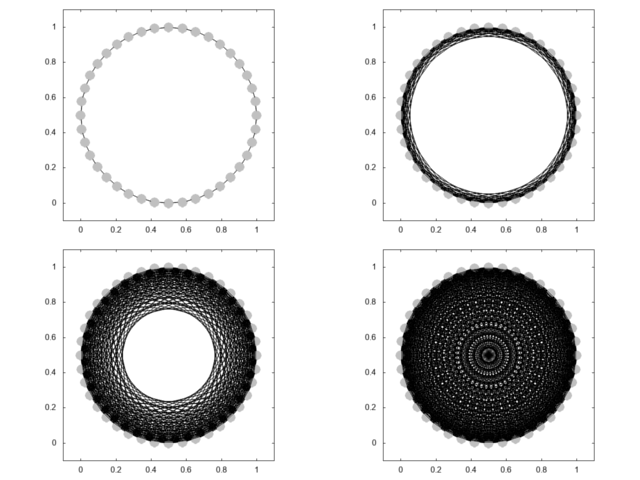
\includegraphics[width=1\textwidth]{grafoEjemplo20}
    \centering
    \caption{Imágenes correspondientes a $k = \{ 1, 6, 13, 20 \}$ en un grafo de cuarenta nodos que forma un polígono regular de cuarenta lados.}
    \label{grafoEjemplo20}
  \end{figure}

  Se implementaron dos algoritmos al código, uno para medir la distancia promedio entre nodos de un grafo y el otro para medir la densidad promedio de un grafo. La \textbf{distancia promedio} se calcula como media de las distancias entre todos los pares de nodos, obtenidas por un algoritmo de Floyd-Warshall. Esta distancia promedio se calcula para cada $k$ y se divide entre $k = 1$ para normalizar la salida, debido a que en $k = 1$ se tiene el promedio de las distancias más largas para cada grafo de este tipo. A su vez, la \textbf{densidad promedio} para cada nodo se calcula a partir de la cantidad de arcos entre sus vecinos entre el total de arcos que podrían establecerse entre sus vecinos, a saber $n (n -1)$ arcos en total. La densidad promedio para el grafo se calcula sumando todas las densidades promedio de los nodos y divididas entre el número de nodos.

  Adicionalmente, se agregó al programa una variable $p$ que representa la probabilidad de que cada nodo se conecte con otro disponible.

  \section{Simulación y resultados}

  Se crearon grafos y se corrieron los algoritmos de distancia promedio y densidad promedio de cada grafo variando $N = \{ 8, 16, 32, 64, 128 \}$ nodos, $k = [1, \lfloor n / 2 \rfloor]$ con $k \in \mathbb{N}$, y $p = (0.2i)_{i= 0}^{25}$ con $p \in \mathbb{R}$. Los resultados se graficaron en una imagen que muestra el comportamiento de la distancia promedio y densidad promedio del grafo frente al incremento de la probabilidad de que se unan los nodos no unidos dado $k$. Se generó una animación que muestra todas las gráficas generadas de esta forma que puede consultarse en \url{https://goo.gl/djPb1X}. Se muestran, además, las figuras de algunas imágenes para discutirlas.

  En las gráficas correspondientes a $N = \{ 16, 32, 64 y 128 \} $, mostradas en la figura \ref{ejemplok1} (p. \pageref{ejemplok1}), muestran una tendencia de las distancias promedio de disminuir de manera exponencial de uno hasta que se alcanzan distancias promedio cercanas a cero cuando la probabilidad de conexión entre nodos no conectados por $k$ es $0.5$. Las densidades promedio siguen una relación lineal que tiende al alza, desde valores cercanos a cero hasta valores cercanos a $1$, $0.5$, $0.25$, $0.125$ respectivamente.

  \begin{figure}[h]
    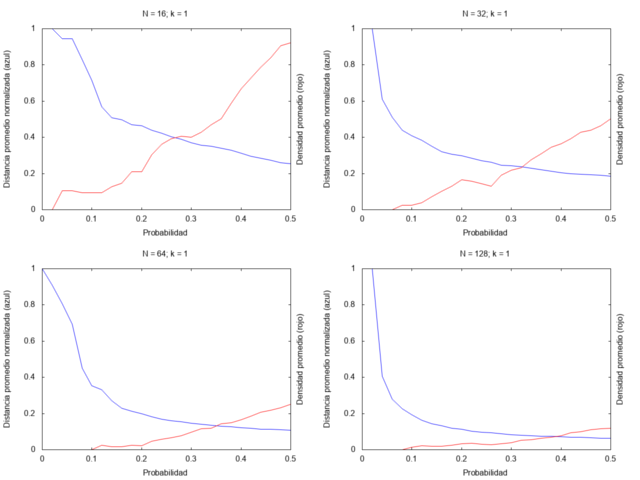
\includegraphics[width=1\textwidth]{ejemplok1}
    \centering
    \caption{Gráficas de distancia promedio (azul) y densidad promedio (rojo) frente a la probabilidad de conexión para grafos con $N = \{ 16, 32, 64, 128 \} $ nodos y $k = 1$.}
    \label{ejemplok1}
  \end{figure}

  Al aumentar la $k$ hasta $N / 4$, es decir, la mitad de los valores de $k$ posibles por $N$ nodos, se obtienen las gráficas de la figura \ref{ejemplokMedia} (p. \pageref{ejemplokMedia}). En dichas gráficas se puede apreciar que las distancias promedio se reducen conforme crece el número de nodos y que las densidades dejan de incrementar para estabilizarse en rangos de $0.6$ y $0.8$. Esto parece deberse a que mientras más nodos hay y más conexiones existen, las distancias entre nodos se minimizan por la cantidad de vecinos que se establecen tanto entre nodos adyacentes como entre nodos situados frente a otros. La densidad, por su cuenta, también se estabiliza pues al crecer el número de nodos, la probabilidad de que se conecten los no conectados por $k$ resulta suavizar la curva.

  \begin{figure}[h]
    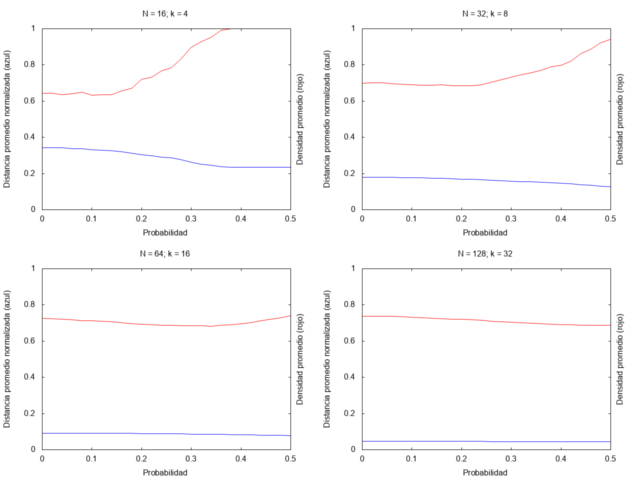
\includegraphics[width=1\textwidth]{ejemplokMedia}
    \centering
    \caption{Gráficas de distancia promedio (azul) y densidad promedio (rojo) frente a la probabilidad de conexión para grafos con $N = \{ 16, 32, 64, 128 \} $ nodos y $k = N / 4$.}
    \label{ejemplokMedia}
  \end{figure}

  La figura \ref{N128k002} (p. \pageref{N128k002}) contiene la gráfica de la simulación con $N = 128$ y $k = 2$, en la que se puede ver la manera en que la probabilidad de establecer vecindades modifica de manera inversa la distancia promedio y la densidad promedio del grafo.

  \begin{figure}[h]
    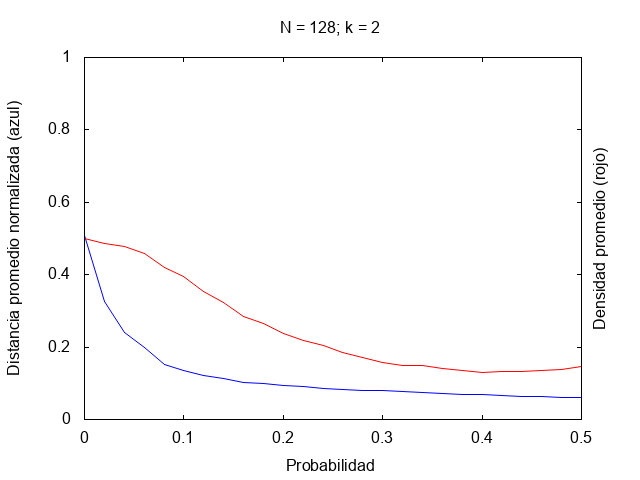
\includegraphics[width=1\textwidth]{N128k002}
    \centering
    \caption{Gráfica de distancia promedio (azul) y densidad promedio (rojo) frente a la probabilidad de conexión para el grafo con $N = 128$ nodos y $k = N / 4$.}
    \label{N128k002}
  \end{figure}

  Finalmente, se comprueba que los tiempos de corrida de las simulaciones crecen de manera exponencial en la figura \ref{Tiempos} (p. \pageref{Tiempos}).

  \begin{figure}[h]
    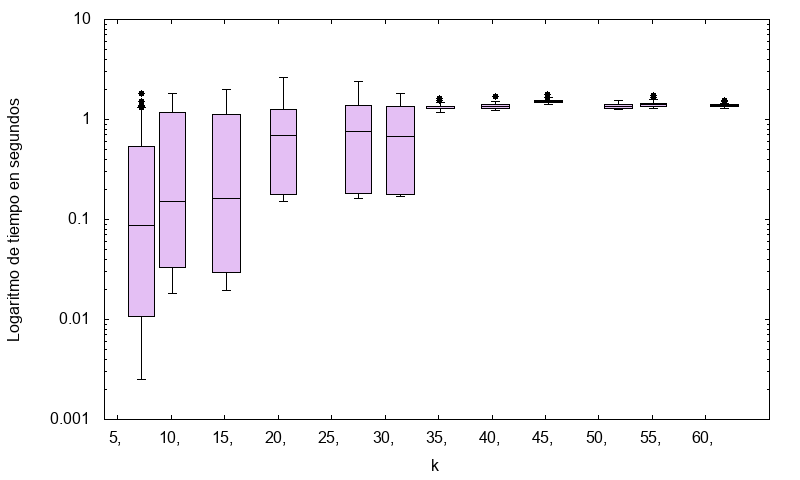
\includegraphics[width=1\textwidth]{Tiempos}
    \centering
    \caption{Gráfica de tiempos de corrida (en segundos) en escala logarítmica contra $k$ para todos los grafos y probabilidades.}
    \label{Tiempos}
  \end{figure}


  \bibliography{biblio}{}
  \bibliographystyle{plain}

\end{document}
